% = = = = = = = = = = = = = = = = = = = = = = = = = = = = = = = = = = = = = = = = = = = = =
% P  R  E  A  M  B  L  E
% = = = = = = = = = = = = = = = = = = = = = = = = = = = = = = = = = = = = = = = = = = = = =
\documentclass[12pt]{article}
\usepackage{amsmath, amssymb, authblk}
%\usepackage{array}
%\usepackage{booktabs}
\usepackage{bm}
\usepackage[small,labelfont=bf,up,singlelinecheck=false]{caption}
%\usepackage{fancyhdr}
%\usepackage[T1]{fontenc}
\usepackage[bottom]{footmisc}
\usepackage{geometry}
\usepackage{graphicx}
\usepackage{hyperref}
%\usepackage[utf8]{inputenc}
	%\inputencoding{latin1}
	%\inputencoding{utf8}
%\usepackage{lettrine}
\usepackage[sc]{mathpazo}
\usepackage{lmodern} % Nice fonts?
%\usepackage{mathrsfs}
\usepackage{mathtools} 
\usepackage{marvosym} % silly bullet-point symbols (misc symbols)
%\usepackage{microtype}
\usepackage{minitoc}         % left in case it is needed elsewhere
\setcounter{secttocdepth}{5} % idem
\usepackage{etoc} % for toc before each section.
%\usepackage{multicol}
\usepackage{needspace}
\usepackage{paralist}
\usepackage{polynom} 			% typesetting polynomial long division
%\usepackage{setspace}
%	\onehalfspacing 
\usepackage[compact]{titlesec} 			% compact shrinks whitespace around section headings.
\usepackage{ulem} 				% for strikeout \sout command.
\usepackage{verbatim}
\usepackage{wrapfig}

% Muh packagez :)
\usepackage{../Packages/MathCommands}
\usepackage{../Packages/BrandonColors}
\usepackage{../Packages/BrandonBoxes}
\usepackage{../Packages/NoteTaker}
\usepackage{../Packages/MachineLearningUtils}


% Title
\title{\vspace{-10mm}\fontsize{24pt}{8pt}\selectfont\textbf{Fall 2016 Course Notes}\vspace*{-4mm}}
% Author
\author{Brandon McKinzie}
% Date
\date{}

% --------------------------------------------------------------
% --------------------------------------------------------------


\begin{document}
\dosecttoc
	

% --------------------------------------------------------------------------
% ==========================================================================
% NEURAL COMPUTATION
% --------------------------------------------------------------------------
% ==========================================================================
\mysection{Neural Computation \\ VS 265}\label{Neural Computation}



% ========================================================
\lecture{Neural Computation}{Sparse Distributed Coding}{September 29}
\begin{itemize}
	\item VI simple-cell receptive fields are localized, oriented, and bandpass. 
	\item PCA is really bad for such situations. 
	\item To detect sharp edges in images, need high frequency and in-phase combinations.
	\item Higher-order image statistics:
	\begin{itemize}
		\item phase alignment
		\item orientation 
		\item motion
	\end{itemize}
	\item want to move beyond pairwise correlations. 
	\item WTA is too greedy, want more distributed strategy. 
	\item Idea: \blue{Projection pursuit}. 
	\begin{itemize}
		\item Look for low-dimensional projections that are as non-Gaussian as possible. 
		\item Projections tend to result in Gaussian distributions by the C.L.T. 
		\item Want to explore projections onto a weight vector until find something Non-Gaussian. Why? Because such a distribution \emph{could not have happened by accident}. 
	\end{itemize}
	\item \blue{Gabor-filter} response histograms are highly non-Gaussian.
	\item (Lab-related) Paper on \textit{Forming sparse representations by local anti-Hebbain learning.}
	\begin{itemize}
		\item Each neuron takes weighted input sum, as well as getting lateral inhibitaion by neighbors, but where the lateral weights are all negative. Put all through $f$, some sigmoidal non-linearity. ''leaky integrator''
		\item Want population-sparcity, so need neurons decorrelated. Have three learning rules: anti-Hebbian, Hebbian, and threshold modification.
		\item Threshold modification resembles homeostasis. 
		\begin{equation}
			\Delta t_i  = \gamma (y_i - p)
		\end{equation}
		which is essentially SGD. Think about average behavior, as it relates to $y_i$ output and $p$. $p$ is a constant to be determined. Feedback loop. Adjusts spiking threshold. 
		\item Anti-hebb guarantees neurons are decorrelated. 
		\begin{align}
			\Delta w_{ij} = \alpha (y_i y_j - p^2)
		\end{align}
		where $p^2$ because this is what we would expected if $i$ and $j$ were decorrelated. There more coactive two neurons are, the more this drives them to repulse one another. 
		\item Standard hebbian rule
		\begin{align}
			\Delta q_{ij} = \beta y_i (x_j - q_{ij})
		\end{align}
		relates to sparsity fraction of neurons. 
	\end{itemize}
	\item Problems:
	\begin{itemize}
		\item Don't know how to deal with graded (i.e. non-binary) input signals. Non-discrete stuff. 
		\item No objective function. Would like way to characterize how well system is performing. 
	\end{itemize}
	\item Led to Bruno's work: \blue{sparse coding for graded signals}
	\begin{itemize}
		\item Data described by
		\begin{align}
			I(x, y) &= \sum_i a_i ~ \phi_i(x, y) + \epsilon(x, y)
		\end{align}
		\item basis decomposition of input. neuron i with activity $a_i$ means that need feature functions $\phi$ to describe model. Want the \blue{neural activities $a_i$ to be sparse}. 
		\item Constrain sparseness of $a_i$ by imposing cost function on the activity:
		\begin{align}
			E = \frac{1}{2} | I - \Phi a|^2 + \lambda \sum_i C(a_i)
		\end{align}
		where first term: preserve information and second term: I want to be sparse. 
		\item Penalty function C shaped like really steep parabola on zero. Or could do $C = |a_i|$, v-shaped thing. 
		\item Energy function determines dynamics of system. Want neuron activity to be expressible as a function of the input $I$. 
		\item Compute coefficients $a_i$ by gradient descent. 
		\begin{align}
			\tau \dot{a_i} = - \frac{dE}{da_i}
		\end{align}
		\item Neuron i inhibited by neuron j proportioanl to their functions $phi$ inner products. 
		\item self-inhibition of neuron back on itself makes it sparse. 
		\item Learning rule:
		\begin{align}
			\Delta \phi_i &= -\eta \frac{\partial E}{\partial \phi_i} \\
			&= \big[I - \Phi \hat{a} \big] \hat{a_i}
		\end{align}
	\end{itemize}
\end{itemize}

% ========================================================
\lecture{Neural Computation}{Foldiak Paper - Sparse Coding}{}
\begin{itemize}
	\item Abstract: A layer of simple Hebbian units connected by modifiable anti-Hebbian feed-back connections can learn to code a set of patterns in such a way that statistical dependency between the elements of the representation is reduced, while information is preserved.
	\item \Part{Introduction}
	\begin{itemize}
		\item Input-space that is our surrounding is enormous, but most inputs are highly correlated, which the brain may exploit to transform the high-dimensional pattern inputs to symbolic representations. Objects may be defined as conjunctions of highly correlated sets of components that are relatively independent of other such conjunctions\footnote{Translation: objects are clumps of stuff that are usually found clumped together, and such that these clumps tend not to clump with other clumps.}
	\end{itemize}
	
	\item \Part{Unsupervised Learning}
	\begin{itemize}
		\item The complexity of the mapping to be learnt $\Leftarrow$ complexity of the input.  
		\item Unsupervised learning exploits statistical regularities in input to learn a more meaningful symbolic representation. 
	\end{itemize}
	\item \Part{The Hebb Unit}
	\begin{itemize}
		\item Simple model of cell (basically perceptron)
		\begin{align}
			y = 
			\begin{cases}
				1 & \sum_j w_j x_j > \text{thresh} \\
				0 & \text{otherwise}
			\end{cases}
		\end{align}
		\item Can be thought of as pattern matching; $y$ is maximal when weight vector = input vector pattern. 
		\item Hebb proposed: connection should become stronger if the two units being connected are active simultaneously: $\Delta w_j = x_j y$. 
	\end{itemize}
	
	\item \Part{Competitive Learning}
	\begin{itemize}
		\item Out of the units receiving weighted sums of the input, only activate the unit with the \emph{largest} weighted sum; suppress the output of all others. 
		\item Results in a local, ''\blue{grandmother-cell}'' representation. 
		\item Limited in number of different inputs it can discriminate, and in ability to generalize. 
	\end{itemize}
	\newpage
	\item \Part{Sparse Coding}
	\begin{itemize}
		\item Distributed coding: instead, code each input state by a \emph{set} of active units (rather than just one). 
		\item Pros: combinatorics of input states increases representational capacity. Cons: situations where many units are active per input pattern, and fact that learning can be extremely slow. 
		\item \blue{Sparse Coding} is a compromise between distributed and local representations. 
	\end{itemize}
	
	\item \Part{Decorrelation}
	\begin{itemize}
		\item Units \textit{within} a layer are connected by modifiable \emph{inhibitory} weights, governed by an \blue{Anti-Hebbian learning rule}: if two units in same layer are active, connection becomes more inhibitory\footnote{which discourages their joint activity}. 
	\end{itemize}
\end{itemize}

% ------------------------------------------------------------------
% COMPREHENSIVE REVIEW VS265
% ------------------------------------------------------------------
\lecture{Neural Computation}{Comprehensive Review}{}

\subsubsection{Unsupervised Learning}
\begin{itemize}
	\item \Part{Bruno:PCA}
	\begin{itemize}
		\item First, let's get this straight. Difference between \blue{covariance} and \blue{correlation}:
		\begin{align}
			\textsc{\red{COV}}[X, Y] &\triangleq \E{(X-\mu_X)(Y-\mu_Y)} \\
			\textsc{\red{CORR}}[X, Y] \equiv \rho_{XY} &\triangleq \dfrac{Cov[X, Y]}{\sigma_X~\sigma_Y}\tlab{corr}
		\end{align}
		
		\item Consider input stream $\matr{x}$ that has linear pairwise correlations\footnote{This is exactly what is meant by eq~\ref{corr}, Pearson's correlation coefficient. \textit{Linear} because ``it is a measure of the linear dependence between two variables X and Y.''} among its elements. Mathematically, correlation between elements $x_i$ and $x_j$ would imply that 
		\begin{align}
			\corr{x_i x_j} = \corrXY{x_i}{x_j} \ne 0
		\end{align}
		or, equivalently, that $\E{x_i x_j} \ne \E{x_i}\E{x_j} = 0$. Bruno is correct that linear pairwise correlations imply that $c_{ij} \ne 0$, he is \textit{absolutely incorrect} to say that $c_{ij}$ is an ``average over many examples.'' That is nothing more than academic sloppiness at its finest. 
	\end{itemize}
	
	\item \Part{HKP:PCA}
	\begin{itemize}
		\item Goal: Find a set of $M$ orthogonal vectors in data space that account for as much as possible of the data's variance. Projecting the data from original $N$-dimensional space onto the $M$-dimensional subspace spanned by these vectors then performs a \textbf{dimensionality reduction}. 
		\item HKP actually states accurately what Bruno meant to state: The $k$th principal component direction is along an eigenvector direction belonging to the $k$th largest eigenvalue of the full \textbf{covariance matrix} 
		\begin{align}
			\corr{(\xi_i - \mu_i)(\xi_j - \mu_j)}
		\end{align}
		
		\item Note: I am now going to start from beginning of CH8 of HKP since I'm not understanding the stuff they are referencing FML
	\end{itemize}
	
	\item \Part{HKP Ch8: Unsupervised Hebbian Learning}
	\begin{itemize}
		\item Units need to learn patterns/correlations/categories in inputs and code the output. Units and connections display some degree of \blue{self-organization}. 
		\item Redundancy provides knowledge: w/o redundancy there would be no patters to learn. 
		\begin{footnotesize}
		\begin{align}
			\text{MaxInfoPossible}-\text{InputContent} = \text{DegreeOfRedundancy}
		\end{align}
		\end{footnotesize}
		
		\item \textsc{\blue{PLAIN HEBBIAN LEARNING.}} Context: output will be continuous-valued and DO NOT have a winner-take-all character\footnote{TODO: Come back and explain why this is true, because current Brandon thought otherwise.}, and so the \red{purpose} is to measure familiarity or projecting onto principal components of input data. 
		\item Setup: Draw at each time step an input vector $\bm{\xi}$ from (multivariate) probability distribution $P(\bm{\xi})$ that has $N$ components\footnote{Confusingly, here $N$ refers to the dimension of space that each input vector lives in (usually denoted by $d$.)}. Network will learn to tell us - as output - how well an input conforms to the distribution\footnote{\red{Q:} Come back and explain why we would want a network to do this. Biological relevance/analog? \green{A}: You need to view it in the context of the grandmother-cell. That's what this is all about. If a given neuron has a large linear output, then we have a good idea of what type of input went in; it was an input really similar to the weight vector. This begs the question, though: how does one determine a reasonable initialization for a given connected layer of weights to a single output? I suppose the answer is that this is the wrong question. Rather, we should interpret the outcome as resulting from a stream of particular inputs and, based on its future responses to inputs, we can determine what type of input went in. With the brain, this is like the jennifer aniston neuron: if that neuron fires, we can assume the person just saw something that resembled Jennifer Aniston.}
		\item (One linear output unit): Let $V$ be a scalar-valued continuous output with a bunch of inputs pointing to it, with 
		\begin{align}
			V = \sum_j w_j \xi_j = \bm{w}^T \bm{\xi} = \bm{\xi}^T \bm{w}
		\end{align}
		\item Want large (on average) $V \leftrightarrow $ more probable $\bm{\xi}$. Why? Because then we can use the relative size of the output as a way of characterizing the sort of input it just received (see footnote 26 below). The weight update to do this is \blue{plain Hebbian learning update:}
		\begin{align}
			\Delta w_i = \eta V \xi_i
		\end{align}
		where it is perhaps easier to think about the situation where $\Delta w_i = 0$ when analyzing, i.e. If $\xi_i = 0$ (which means it had nothing to do with the output), then don't increase it's weight\footnote{Minor TODO: Analyze case of non-binary (i.e. continuous both pos/neg) inputs/outputs.}. 
		\item Problem: $\bm{w}$ grows without bound. However, suppose stable equilib exists for $\bm{w}$. This could happen for example, when considering that the update just performs $\bm{w} = \eta V \bm{\xi}$, where eventually $||\bm{w}|| >> ||\bm{\xi}||$ in addition to the fact that $\xi$ is quite likely to be along $\bm{w}$. So at equilib, expect the updates to average to $0$:
		\begin{align}
			0 &= \corr{\Delta w_i} \\
			&= \corr{\sum_j w_j \xi_j \xi_i} \\
			&= \sum_j \matr[ij]{C} w_j
		\end{align}
		where the brackets are \textit{expectation values} in the sense that 
		\begin{align}
			\corr{\xi_i \xi_j} = \iint_{-\infty}^\infty \xi_i \xi_j f_{\xi_i \xi_j}(\xi_i, \xi_j) d\xi_i d\xi_j 
		\end{align}
		where $f$ is the PDF for the two random variables in question. I suppose that, since strictly speaking $\bm{w}$ isn't a random variable, that it can be pulled out along with the summation. That satisfies me for now. 
		\item Given that $\bm{\xi}$ can be interpreted as a column vector, we have
		\begin{align}
			\matr[ij]{C} &\equiv \corr{\xi_i \xi_j} \\
			\matr{C} &\equiv \corr{\bm{\xi}\bm{\xi}^T}
		\end{align}
		Now, to be perfectly clear, this is NOT the correlation, but I am so sick and tired of caring that I'm just going to accept their absolutely incorrect definition and move on. 
		\item Since I've read ahead, I know that the following property will be important to remember:
		\begin{align}
			\forall \bm{x},~ \bm{x}^T \matr{C} \bm{x} 
			&= \bm{x}^T \corr{\bm{\xi}\bm{\xi}^T}\bm{x} \\
			&= \corr{\bm{x}^T \bm{\xi}\bm{\xi}^T\bm{x}}\\
			&=  \corr{(\bm{\xi}^T\bm{x})^2}
		\end{align}
		\item There are \textit{only} unstable fixed points (unstable equilib) for the plain Hebbian learning procedure. 
		
		
		\item \blue{\textsc{OJA'S RULE}}. Goal: Modify plain Hebb rule such that $|\bm{w}| = 1$. 
		\item Solution: Add a \green{weight decay} proportional to $V^2$:
		\graybox{\Delta w_i = \eta V (\xi_i - V w_i )}
		and we see that $\Delta w$ depends on the difference between the input and the back-propagated output\footnote{Say 'back-propagated output' because we are subtracting what was put into the network by the resultant output \textit{times} the connection (weight) between the input and said output. Dwelling on this \textit{would} be overly pedantic, so move on.}
		\item Informal analysis for zero-mean data: The average component of $\xi$ along $w$ will be zero, but since this is an algorithm depending on an unstable equilibrium, it will tend to fall along the maximal eigenvector of $\matr{C}$. 
		\item Oja's rule chooses the direction of $\bm{w}$ to maximize $\corr{V^2}$. 
		
		
		\item \blue{\textbf{Sanger's Learning Rule}}. Setup: Now, instead of 1 output, have $M$ output neurons with the hopes that they gives us the first $M$ principal components of the input data. Architecture is ONE LAYER fully connected. 
		\item The ith output is a linear neuron as usual given by
		\begin{align}
			V_i = \sum_j w_{ij} \xi_j = \bm{w}_i^T \bm{\xi} = \bm{\xi}^T \bm{w}_i
		\end{align}
		\item The Sanger's learning rule update for the connection \textit{from} the $j$th input component \textit{to} the $i$th output neuron (so we are only updating a single edge/line in the following) is
		\graybox{\Delta w_{ij} = \eta V_i \bigg(\xi_j - \sum_{k=1}^{i} V_k w_{kj} \bigg)}
		where the (converged) weight vectors to the output neurons are orthonormal and converge to the normalized eigenvectors in order of largest to smallest eigvals:
		\begin{align}
			\bm{w}_i^T \bm{w}_j &= \delta_{ij} \\
			\bm{w}_i &\rightarrow \pm \bm{c}^{i}
		\end{align}
	\end{itemize}
\end{itemize}

\lecture{Neural Computation}{Lab 4 \& LCA Handout}{}
\begin{itemize}
	\item Want to learn a ``dictionary'' from data
	\item Encode input data such that it can be reconstructed from that code, where dim(encoding) > dim(input). 
	\item Given $N$-dimensional input, build $N\times M$ dictionary\footnote{M > N.} (matrix) $\matr{\Phi}$ where each column $\phi_i$ is a dictionary element with corresponding coefficient\footnote{Looks like $a_i \notin \matr{\Phi}$} $a_i$. Want to assemble $a_i \phi_i$ into a vector of \blue{activations}.  
	\item \textbf{GOAL:} Minimize energy function $E$, defined as 
	\graybox{E = \onehalf ||S - \hat{S} ||_2^2 + \lambda \sum_i^M C(a_i) }
	where $\hat{S} = \sum_i^M a_i \phi_i$ is for some reason called the image reconstruction. View this like a regularization procedure where the terms mean: (1) smallest difference between true image and reconstructed image (\blue{reconstruction quality}); and (2) limit the number of \blue{active elements}\footnote{A.k.a sparsity constraints a.k.a limit activations.} $a_i$. 
	
	\item Want to minimize $E$ such that reconstructs data with fewest number of active elements, expressed as 
	\begin{align}
		\argmin_{a,~\matr{\Phi}} \big( E \big) \tlab{argminE}
	\end{align}
	where I guess the double argmin means "minimize E by changing $a$ and $\matr{\Phi}$ only and then give me the values of $a$ and $\matr{\Phi}$. 
	
	\item Popular cost function is the $\ell_1$ penalty: 
	\begin{align}
		\sum_i^M C(a_i) = \sum_i^M  |a_i|
	\end{align}
	
	\item We compute coeff vector $a$ using a ``dynamic process''\footnote{Okay well what the fuck is it?} that minimizes~\ref{argminE}. 
	
	\item Method for computing the sparse code from a given input signal $S$ and dictionary element $\phi_i$ is the \blue{Locally Competitive Algorithm}. 
	\begin{quote}
		The model describes an activation coefficient, $a_k$, as the thresholded output of some model neuron's \textbf{internal state}, $u_k$, which is analogous to the neuron's
		membrane potential.
	\end{quote}
	
	\item Here we compute the equation for state transitions (updates) from the energy function. First, for grad descent on an individual neuron's activity, $a_k(t)$:
	\graybox{-\pderiv{E(t)}{a_k(t)} = 
		\sum_i^N\bigg[S_i\Phi_{ik} - \sum_{j\ne k}^{M} \Phi_{ik} \Phi_{ij} a_j\bigg]
		- a_k - \lambda \pderiv{C(a_k)}{a_k}}
	where the constants are $S$ and $\matr{\Phi}$. Want system to evolve over time to produce optimal set of activations $a(t)$. 
	
	\item Meaning of $\phi_k$. Associated with $k$th (output?) neuron. Indicates the connection strength [between that neuron and] each pixel in the input. 
	
	\begin{quote}
		In this model, we are going to nd a sparse code for one patch of an image
		at a time, so that all M neurons are connected to the same image patch, S.
	\end{quote}
\end{itemize}


\lecture{Neural Computation}{HKP 9.4 - Feature Mapping}{}

\p Nearby (similar) outputs corresponding to nearby (similar) input patterns. Such a map (similar inputs $\rightarrow$ similar outputs) is a \blue{feature map}. The conventional case: 2 continuous-valued inputs $x$ and $y$ map (fully-connected) to a two-dimensional x,y grid. Want nearby input values (in the actual euclidean sense) (x, y) to be mapped closely in the output 2D grid. \\

\p \blue{Kohonen's Algorithm} implements the self-organizing (feature) map by using competitive learning, where now we update weights going to the \textit{neighbors} of the winning unit as well as those of the winning unit itself. 
\begin{itemize}
	\item Setup: $N$ continuous-valued inputs $\xi_1$ to $\xi_N$, defining a point $\bm{\xi}$ in $N$-dimensional space. Outputs $O_i$ are arranged in (typically) a 1-D or 2-D array fully connected via $w_{ij}$ to the inputs. 
	
	\item A competitive learning rule is used, choosing output $O_i^*$ as winner, determined by
	\begin{align}
		|\bm{w_i^*} - \bm{\xi}| \le |\bm{w}_i - \bm{\xi}| ~~ \mgreen{\text{(for all i)}}
	\end{align}
	
	\item The \blue{Kohonen Learning Rule} is 
	\graybox{\Delta w_{ij} = \eta \Lambda(i, i^*)(\xi_j - w_{ij})}
	where $\Lambda(i, i^*)$ is the \textbf{neighborhood function}, equal to 1 for $i = i^*$ and falls off with distance $|\bm{r} - \bm{r_i}^*|$. 
	
	\item A typical choice for $\Lambda(i, i^*)$ is
	\begin{align}
		\Lambda(i, i^*) = \exp\bigg(- \frac{|\bm{r} - \bm{r_i}^*|^2}{2 \sigma^2} \bigg)
	\end{align}
	where $\sigma$ is width parameter that \textit{is gradually decreased}. Apparently $\eta(t) \propto t^{-\alpha}$ where $0 < \alpha \le 1$ is a good choice. 
\end{itemize}



%
%
%
\lecture{Neural Computation}{Locally Linear Embedding}{October 19}

LLE is an unsupervised learning algorithm for dimensionality reduction. Similar to PCA and MDS\footnote{Multidimensional scaling}, LLE is called an \textit{eigenvector method}. The basic idea is illustrated below in figure~\ref{LLE}. \\

% --------------- FIGURE : LLE.PNG -------------------
\begin{figure}[b!]
	\centering
	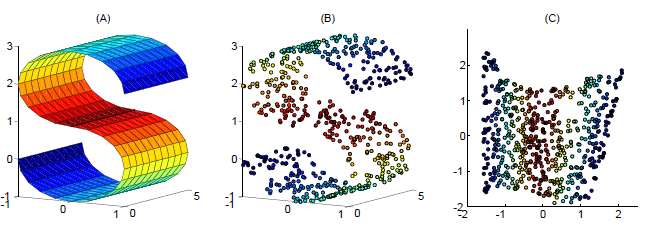
\includegraphics[]{LLE.PNG}
	\caption{(A) Multidimensional sampling distribution with clear underlying manifold representation. (B) Points that were sampled. (C) The neighborhood-preserving mapping discovered by LLE. }
	\label{LLE}
\end{figure}

\p The \textbf{LLE algorithm}:
\begin{enumerate}
	\item Compute the neighbors of each data point, $X_i$. 
	\item Compute the weights $W_{ij}$ that best reconstruct each $X_i$ from its neighbors, minimizing the cost in
	\graybox{ 
		ReconErr(W)  = \sum_i | X_i - \sum_j W_{ij} X_j |^2 \label{ReconErr}
	}
	by constrained linear fits. 
	\item Compute the $Y_i$ reconstructed by the weights $W_{ij}$, minimizing the quadratic form in
	\graybox{
		\Phi(Y) = \sum_i |Y_i - \sum_j W_{ij} Y_j |^2 \label{map}
	}
	by its bottom nonzero eigenvectors. 
\end{enumerate}

\p Some intuition/overview of the algorithm. We expect each $X_i$ and its neighbors to lie on or close to a \blue{locally linear} patch of the manifold. We characterize these patches by linear coefficients $W_{ij}$ that reconstruct each $X_i$ from its neighbors. As seen in eq.~\ref{ReconErr}, the reconstructed point $X_i$ is given by $\sum_j W_{ij} X_j$.  \\

\p \textbf{Computing/analyzing the weights $W_{ij}$}. Minimize eq~\ref{ReconErr} subject to 
	\begin{align}
		\forall X_j \notin \text{Neighbors}(X_i) ~ : ~ &W_{ij} = 0 \\
		\sum_j ~ &W_{ij} = 1 
	\end{align}
where the optimal weights are found by solving a least squares problem. Note that for a given data point, \textit{the weights are invariant to rotations, rescalings, and translations of that data point and its neighbors.}\footnote{In other words, since the weights just characterize the local patch of the given data point, that patch shouldn't change if we shift the data, rotate it, or scale it. The neighboring points should remain the same.} If the data lie on some nonlinear manifold of $d << D$, then there exists a \textit{linear mapping} (approx) from the high-D coordinates of each neighborhood to global ('internal') coordinates on the manifold. Lucky for us, $W$ can also do this!\footnote{In particular, the same weights $W_{ij}$ that reconstruct the $i$th data point in D dimensions should also reconstruct its embedded manifold coordinates in d dimensions} \\

\p \textbf{Explanation of eqs.~\ref{ReconErr}~\ref{map}}. Note that eq.~\ref{ReconErr} is minimized over the $W_{ij}$, while equation~\ref{map} is minimized over the $Y_i$. In English: We first want the weights $W$ that reconstruct each $X_i$ by its neighbors in the high-D space. Then, we want the low-$d$ coordinates $Y_i$, representing the global coordinates on the manifold, that correspond to each $X_i$ from the original space. \textbf{How it is minimized:}
	\begin{quote}
		it can be minimized by solving a sparse $N \times N$ eigenvector problem, whose bottom $d$ non-zero eigenvectors provide an ordered set of orthogonal coordinates centered on the origin.
	\end{quote}
	
\p \textbf{Implementation of algorithm.} Only one free parameter: number of neighbors per data point $K$. $W_{ij}$ and $Y_i$ are computed by 'standard linear algebra'. 

% =========================================================================
% RECURRENT NEURAL NETWORKS
% =========================================================================
\lecture{Neural Computation}{Recurrent Neural Networks}{October 20}

\p \blue{Lab 6 Overview}. Briefly goes over how we can corrupt some number of bits and reconstruct a desired image [with hopfield nets]. Unfortunately, can get ``spurious basins of attractions.'' Pushing down on some region of landscape causes pushing up of some other region. Want to carve energy landscape so that we push down only where we want. \\

\p \blue{Bump circuits and ring attractors}. Want family of solutions (e.g. a line) that solutions drawn to (called line attractors). Head-direction neurons\footnote{Literally referring to direction of [e.g. some animal's] head} look like an internal compass for animals; encode direction of head in \textit{world coordinate system}. Different dots represent a single neuron's firing rate at different relative head directions. \textbf{Ring attractors}: population of neurons that with bumps that are stable (?). Convergence/stability because $T_{ij}$ matrix is symmetric. Symmetric = fixed stable; Asymmetric =  \\

\p Bruno shows simulation:
\begin{compactitem}
	\item 32 neurons where bar is activity of neuron. 
	\item Start with random symmetric weight hopfield net.
	\item Eventually weights converge to gaussian-like bump; an equipotential pattern. 
	\item If we add small asymmetry (gamma) to weights, then population (bump) would shift. Bump change is shifting position, and when the asymmetry stops (we stop moving our head) the population stays fixed. In English: moving head causes bump to move but when we stop moving, they stay put. 
	\item \green{For more}: Read "catcher and zong" paper. I misspelled that. 
\end{compactitem}
\myspace

\p [\textit{Enter guest lecturer Alex Anderson}] \Part{Recurrent Neural Networks}: 
\begin{compactitem}[$\rightarrow$]
	\item Starts with handwriting network. 
	\item RNNs good for sequence prediction tasks with ``long-term dependencies.''
\end{compactitem}

\Needspace{10\baselineskip} 
\p \blue{Backprop Review}. Blobs do activation computation and transformers do propagations. Note: $A^t$ is target output values. \\

\p \blue{Problem to Solve}. Feed net a bunch of sentences and have it fill in the blank somewhere, based on the previous info it was fed. Mad libs. Have network understand particular frame of movie by exploiting context; just showing it a bunch of frames isn't enough/good approach. \\

\p \blue{RNN loops/Notation}. Feed \textit{time sequence} $x_t$ to block $A$. Two figures in this slide are different reps of same thing; instructor prefers the right fig. $H_k$ is hidden state we want to predict\footnote{Analogy to hopfield: H is like hopfield B. X is like external I in hopfield.}. $f$ can be some nonlinearity like $tanh$. In RNNs, cost function typically broken up over time; so $C_k$ is cost at timestep $k$. Usually want hidden state to \textit{summarize} the past. Hidden state traces out a trajectory over time [wut]. \\

\p \blue{Unroll a RNN}. Can basically turn RNN into a linearized hidden markov chain, where time proceeds to the right. Total cost is given by cost at each time step. \\

\p \blue{Long-term Dependencies}. Shows toy model. Imagine ur an ant walking along graph. Given string of nodes, predict next letter each timestep [solve the question mark in slide]. Don't necessarily want/need whole past as input. Want to remember past [hidden] states, but they usually get overwritten; want to save it more efficiently. Key: want to make function simple, give the network parameterization. \\

\p \blue{Exploding/vanishing gradients}. Local dependencies easy to learn. 
\begin{compactitem}[$\rightarrow$]
	\item Once we get to B, want network to output a U. 
	\item To learn, errors need to propagate back [in time], so we can change the weights that started the error: gradient of cost at timestep $k$ with respect to initial weights using chain rule. Basically a product of $k$ matrices. 
	\item If $k$ large and matrices have eigvals less than 1, gradients \textit{vanish}. If eigvals above 1, gradients \textit{explode}. So what we want is for eigvals to be very near 1. 
	\item \red{Todo}: lookup relationship between eigval magnitudes and determinant. 
\end{compactitem}

\Needspace{10\baselineskip}
\p \blue{Solution: Multiplicative Gating}. Helps protect hidden state. MultGate can be either 0 or 1, and we multiply the hidden state by that value; if we 0 lose the hidden state; if 1 we keep the hidden state. Since binary functions not smooth/differentiable, continuous gating is better. [slide note: top row is w/o multgate, lower row is with multgate]. Key equation: $$ c_t = f_t \odot c_{t - 1} + i_t \odot j_t$$ where $\odot$ is elementwise product. \\

\p Note: This is in TensorFlow now. 

% =========================================================================
% RECURRENT NEURAL NETWORKS
% =========================================================================
\lecture{Neural Computation}{Hopfield Networks Handout}{October 26}

\p \blue{Energy Function}. The following governs the dynamic of pairwise recurrently connected networks. 
\graybox{E = \onehalf \sum_i \sum_{j\ne i} T_{ij} V_i V_j }
For symmetric weights $T_{ij} = T_{ji}$, consider the change in energy $\Delta E$ resulting from making a positive change to $V_k$\footnote{If it is -1, change to +1, else just keep where it is.}
\begin{align}
\Delta E = -\Delta V_k \sum_{i \ne k} T_{ki} V_i
\end{align}
which will be \textit{negative} if both $\Delta V_k$ and the sum are positive, thus decreasing the overall energy (good). Conversely, if sum is negative, we should decrease value of $V_k$. \textbf{Critical assumption}: Symmetric $T_{ij} = T_{ji}$. Without this assumption, impossible to show the system will have fixed points. 
\begin{quote}
	For a network with symmetric
	connections though, the dynamics will converge to so-called \blue{basins of attraction}.
\end{quote}
\myspace

\p \blue{Setting the Weights}. Goal: store pattern $\matr{V}^\alpha$ as basin of attraction in network. One approach: the \green{Hebbian prescription} $T_{ij} = V_i^\alpha V_j^\alpha$.
\begin{itemize}[$\rightarrow$]
	\item \textbf{Single memory storage}. Now, the summed input sent to, say, the $i$th unit in response to some  $\matr{V}^\beta$ will be given by 
	\begin{align}
		U_i = V_i^\alpha \sum_{j \ne i} V_j^\alpha V_j^\beta 
	\end{align}
	and thus if  $\matr{V}^\alpha = \matr{V}^\beta$, $U_i$ won't flip sign and the networks stays put.
	
	\item \textbf{Multiple memories}. Now, need to form as many basins of attractions as memories we want stored. Set weights with a superposition over each desired \textit{memory} $\matr{V}^\alpha$: $T_{ij} = \sum_\alpha V_i^\alpha V_j^\alpha$, and the corresponding response of the $i$th neuron is
	\begin{align}
		U_i = \sum_\alpha V_i^\alpha \sum_{j \ne i} V_j^\alpha V_j^\beta \label{18}
	\end{align}
\end{itemize}

\p \green{Capacity for a Hopfield Network}. If the patterns to store (memories) have \textit{few elements in common}, then cross terms $\sum_{j\ne i}  V_j^\alpha V_j^\beta$ tend to zero for $\alpha \ne \beta$ (since each $V_j^\alpha$ is $\pm 1$ and a random average over $\pm 1$ is zero) and $U_i$ won't change. As we store more patterns which are \textit{similar}, memories degrade and basins gone from desired locations. This \textbf{capacity} for Hopfield is $\approx 15\%$ of the number of neurons in network\footnote{Assuming the stored patterns are relatively dissimilar.}.





% =========================================================================
% RECURRENT NEURAL NETWORKS
% =========================================================================
\lecture{Neural Computation}{Mixture of Gaussians and EM Algorithm}{November 3}

\p \blue{(MOG) Model Assumptions}. Assume each $x^{(i)}$ generated by sampling $z^(i) \sim Multinom(\phi)$\footnote{where k-vector $\phi$ elements $\phi_j = P(z^{(i)} = j)$} and then positing that $x^{(i)}$ was drawn from the Gaussian associated with $z^{(i)}$ (so $k$ possible Gaussians since $z$ could be one of $k$ classes), i.e. 
\graybox{x^{(i)} | z^{(i)} = j \sim \mathcal N(\mu_j, \Sigma_j) }

\myspace
\p \blue{Goal}. Estimate the parameters of our model, $\phi, \mu, \Sigma$. We can do this by writing the likelihood of our data ($m$ data points):
\begin{align}
\ell(\phi, \mu, \Sigma) &= \sum_{i = 1}^{m} \log\left[
	\sum_{z^{(i)} = 1}^k p\left( x^{(i)} | z^{(i)} ; ~ \mu, \Sigma\right)~p(z^{(i)}; \phi)
 \right]
\end{align}
where the inner sum comes from using Bayes rule on $p(x^{(i)})$. Note that \textit{we don't know the $z{(i)}$ for each data point}, that information is hidden. This means we can't get closed-form solutions by doing MLE/taking derivatives as usual.

\myspace
\p \blue{EM Algorithm}. Purpose: allow us to move forward given we can't do the standard MLE approach (since we don't know the values of each $z^{(i)}$.)
\begin{enumerate}
	\item \textbf{E-step}. Estimate the values of the $z^{(i)}$s by evaluating
	\begin{align}
		\text{For each $i, j$, set } w_j^{(i)} := p(z^{(i)} = j~|~ x^{(i)}; ~ \phi,\mu,\Sigma)
	\end{align}
	with Bayes' rule, using whatever the current values of the estimated parameters are. 
	
	\item \textbf{M-step}. Update parameters via standard MLE approach. 
	\begin{align}
	\phi_j &:= \frac{1}{m} \sum_{i = 1}^m w_j^{(i)} \\
	\mu_j &:= \dfrac{ \sum_{i = 1}^m w_j^{(i)} x^{(i)} }{ \sum_{i = 1}^m w_j^{(i)}  } \\
	\Sigma_j &:= \dfrac{ \sum_{i = 1}^m w_j^{(i)}(x^{(i)} - \mu_j) (x^{(i)} - \mu_j)^T }{ \sum_{i = 1}^m w_j^{(i)}  } 
	\end{align}
\end{enumerate}

Some properties of the EM-algorithm. It is similar to the K-means algorithm, and like K-means, it is also prone to local minima, so reinitializing at several different initial parameters may be a good idea. 



% =========================================================================
% BOLTZMANN MACHINES
% =========================================================================
\lecture{Neural Computation}{Boltzmann Machines}{November 6}

\hrule
\subsubsection{Lecture Slides}
\hrule
[Here, I use my own notation that actually remains consistent/intuitive...]

The energy, taken as a sort of average over all pairwise connections and the corresponding network-wide probability is
\graybox{
	E(\bm{s}) &= - \onehalf \sum_{ij} w_{ij} s_i s_j \\
	P(\bm{s}) &= \frac{1}{Z} e^{- \beta E(\bm{s}) }
	}

\myspace
\hrule
\subsubsection{HKP Chapter 7.1}
\hrule
\p \blue{Structure}. The units $S_i$ are divided into 
\begin{enumerate}
	\item \textbf{Visible units}. These may be further divided into, e.g., input and output units.
	\item \textbf{Hidden units}. No connection to the outside world. 
\end{enumerate}
\begin{figure}[h!]
	\centering
	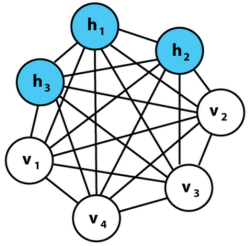
\includegraphics[height=0.15\textwidth]{boltzmann.PNG}
	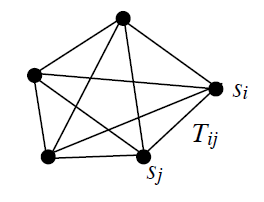
\includegraphics[height=0.15\textwidth]{boltzmann2.PNG}
\end{figure}

\p The units are \blue{stochastic}, meaning 
\begin{align}
S_i &= 
\begin{cases}
	+1 & \text{with probability } g(h_i) \\
	-1 & \text{with probability } 1 - g(h_i)
\end{cases}\\
h_i &= \sum_j w_{ij} S_j \\
g(h) &= \frac{1}{1 + \exp(-2\beta h)}
\end{align}
where $\beta = 1/T$ and $T$ is the ``temperature.'' \textbf{Goal:} adjust the weights $w_{ij}$ to give the states of the \textit{visible} units a particular desired probability distribution. This differs from a Hopfield network in that now we have hidden units. With hidden units, we can specify \textit{higher-order correlations} between units\footnote{Whereas, in hopfield networks, we can do no more than specify all the $\langle S_i \rangle$ and $\langle S_i S_j \rangle$}. 


\myspace
\hrule
\subsubsection{Boltzmann Machines - AIFH}
\hrule

\myspace
\p A Boltzmann machine is essentially a fully connected, two-layer neural network; one visual layer and one hidden layer. \textbf{Restricted} Boltzmann machines are not fully connected; all hidden neurons are connected to each visible neuron and vice versa, but there are no connections between neurons of the same layer. 
\begin{compactitem}
	\item Boltzmann machines are a generative model. 
	\item The values presented to the visible neurons of a Boltzmann machines, when considered with the weights, specify a probability that the hidden neurons will assume a value of 1, as opposed to 0. 
\end{compactitem}


\myspace
\p \blue{Differences with Hopfield networks}. 
\begin{compactitem}[$\rightarrow$]
	\item Hopfield networks suffer from recognizing false patterns.
	\item BM can store a greater capacity of patterns than HN.
	\item HN require the input patterns to be uncorrelated.
	\item BM can be stacked to form layers.
\end{compactitem}




% =========================================================================
% BOLTZMANN MACHINES
% =========================================================================
\lecture{Neural Computation}{Independent Component Analysis}{November 12}

\hrule
\p \blue{Sparse Coding Review}. The goal is to represent input $x$ as vector of sparse coefficients $s$, where their relationship is given in the form 
\begin{align}
\bm{x}= \matr{A} \bm{s} + \bm{n}
\end{align}
\begin{compactitem}[$\rightarrow$]
	\item \blue{$\bm{x}$}: Data matrix with shape $n$ by $d$. 
	\item \blue{$\matr{A}$}: Feature matrix (contains the basis functions) of shape $n$ by $k > n$. Here, $k$ is the number of sparse coefficents (shape of $\bm{s}$). 
	\item \blue{$\bm{s}$}: The sparse coefficient matrix. Recall that the equation above is sometimes written as a sum over the basis functions $\phi$.
	\begin{align}
		\bm{x} = \left(\sum_k \phi_k (\bm{x})s_k\right) + \bm{n} 
	\end{align}
	We say ``sparse'' because $s_i = 0$ a lot, and $\text{shape}(\bm{s}) > \text{shape}(\bm{x})$. 
	\item \blue{$n$}: Gaussian noise. Entries are typically much smaller than entries of $\matr{A}\bm{s}$.
\end{compactitem}
\hrule



\myspace
\begin{itemize}
	\item \textbf{Model distribution.}
	\begin{align}
		p(\bm{x}) &= \int p(\bm{x} | \bm{s}) p_s(\bm{s})d\bm{s} \qquad \text{where}\\
		p(\bm{x} | \bm{s}) &\propto e^{-\frac{|\bm{x} - \matr{A}\bm{s}|^2}{2\sigma^2_n}} \qquad \text{and}\\
		p_s(\bm{s}) &\propto e^{-\sum_i C(s_i) } \quad \leftrightarrow \quad \matr{C} = -\log(p(\bm{s}))
	\end{align}
	
	\item \textbf{Learning Rule}. 
	\begin{alignat}{2}
		\Delta\matr{A} 
		&\propto \pderiv{}{\matr{A}}\left<	 \log p(\bm{x}) \right> \\
		\Delta\matr{A} 
		&\propto \left<	 \int [\bm{x} - \matr{A}\bm{s}] \bm{s}^T \mred{ p(\bm{s}|\bm{x}) }d\bm{s}	 \right> \qquad &&\textsc{(Analytic)} \\
		\begin{split}
		\Delta\matr{A} 
		&\propto \left<	 [\bm{x} - \matr{A}\bm{\hat s}] \bm{\hat s}^T\right> \qquad
		\end{split}&&\textsc{(In Practice)} 
	\end{alignat}
	where, $\bm{\hat s}$ represents a single sample at the posterior maximum: 
	\begin{align}
	\bm{\hat s} &= \argmax_s p(\bm s|\bm x) \\
	&= \argmin_s \left[ -\log(p(\bm{s}|\bm{x})) \right] \\
	&= \argmin_s \left[ \frac{\lambda_n}{2} |\bm x - \matr{A}\bm s |^2 + \sum_i C(s_i) \right] \\
	\nabla_s  \bm{\hat s} 
	&\propto \lambda_n \matr{A}^T [\bm x - \matr{A} \bm s] - C'(\bm{s}) \\
	&\triangleq \lambda_n [\bm b - \matr{G} \bm s] - \bm z (\bm s)
	\end{align}
\end{itemize}

\myspace
\p \blue{Independent Component Analysis}. Special case where (1) $\matr{A}$ is square and full rank, and (2) the noise $\bm{n} = 0$. Now we have model
\begin{align}
\bm{x} = \matr{A}\bm{s} \quad \rightarrow \quad \bm{s} = \matr{A}^{-1}\bm{x}
\end{align}

\textbf{Learning rule}.
\graybox{
	 \Delta\matr{A} &\propto \left<	 [\bm{x} - \matr{A}\bm{\hat s}] \bm{\hat s}^T\right>  \\
	\Delta \matr{A} &\propto \matr{A}\left< \bm{z}(\bm{s}) \bm{s}^T \right> - \matr{A}
	}


\myspace
\p \blue{Equations for Different Priors}

\begin{alignat}{3}
	&\mred{\textsc{[LAPLACE]}} \qquad P(s_i) &\propto e^{-|s_i|} \quad \leftrightarrow \quad z_i &&= \text{sign}(s_i) \\
	&\mred{\textsc{[CAUCHY]}} \qquad P(s_i) &\propto \frac{1}{1+s_i^2} \quad \leftrightarrow \quad z_i &&= \frac{2|s_i|}{1 + s_i^2} \\
	&\mred{\textsc{[GAUSS]}} \qquad P(s_i) &\propto e^{-s_i^2}{2} \quad \leftrightarrow \quad z_i &&= |s_i| 
\end{alignat}

\myspace\Needspace{10\baselineskip}
\p \blue{Algorithm summary/procedure}. 
\begin{compactitem}
	\item[1.] Initialize square matrix $A$. 
	\item[2.] Until $A$ converges, do:
	\begin{compactitem}
		\item Compute source vector via $\bm{s} = \matr{A}^{-1}\bm{x}$. 
		\item Compute 
		\begin{align}
			\bm{z} 
			&= \nabla_{s} C(\bm{s}) \\
			&= \nabla_{s} \left[- \log(p(\bm{s})) \right]  \\
			&= - \sum_{i} \nabla_{s} \log(p_s(s_i))
		\end{align}
		
		\item Update
		\graybox{
			\Delta A \propto A \left< \bm{z}(\bm{s}) \bm{s}^T \right> - A
		}
		
	
	\end{compactitem}
\end{compactitem}









\myspace
\Needspace{10\baselineskip}
\hrule
\subsubsection{ICA - Andrew Ng - CS 229}
\hrule 

\myspace 
\p \blue{Cocktail Party}. There are $n$ people talking at a cocktail party, and we've placed $n$ microphones in the room to see if we can separate out the original $n$ speakers' speech signals. We observe
\begin{align}
x = As
\end{align}
\begin{compactitem}[$\rightarrow$]
	\item $x^{(i)}$ denotes the $n$-dimensional vector of our microphone recordings at time $i$. 
	\item $s^{(i)}$ denotes the $n$-dimensional vector of each speakers' output at time $i$. 
	\item $A$ be the unknown square \textbf{mixing matrix}. \textbf{Goal}: Find the \textit{unmixing matrix} $W = A^{-1}$. Then we can recover the generated sources via $s^{(i)} = W x^{(i)}$. 
	\graybox{
	\begin{split}
		W = \begin{bmatrix}
			- & w_1^T & - \\
			- & w_2^T & - \\
		 & \vdots &  \\
			- & w_n^T & - 
		\end{bmatrix}
	\end{split}
	\qquad\qquad\longrightarrow\qquad 
	\begin{split}
		s_j^{(i)} = w_j^T x^{(i)}
	\end{split}
		}
\end{compactitem}
\red{[ELI5]} ``People say stuff $s^{(i)}$, but it gets all mixed up so we hear stuff $x^{(i)}$. We want to know how they related. Luckily, we can just unmix the mixed stuff.''

\myspace
\p \blue{Ambiguities}. The (1) order and (2) scaling of the $n$ ``$w_i$'' vectors in $W$ is ambiguous. The sign of $s_j^(i)$ is irrelevant (sounds the same on a speaker). \textbf{Key point}: The aforementioned ambiguities are the \textit{only} ambiguities, so long as the sources $s_i$ are \textit{non-Gaussian}. Basically, this is due to things like rotational invariance that can be present in Gaussians.


\myspace
\p \blue{ICA Algorithm}. 
\begin{enumerate}
	\item Let each source $s_i$ have density $p_s(s_i)$. Then the joint distribution $p(s)$ is the probability of hearing all independent sources $s_i$. From previous results, we know that this implies a density for $x = As = W^{-1}s$ (below). 
	\begin{align}
		p(s) = \prod_{i = 1}^{n} p_s(s_i) \quad \implies \quad
		p(x) = \prod_{i = 1}^{n} p_s(w_i^T x) \cdot |W|
	\end{align}
	
\end{enumerate}

% --------------------------------------------------------------------------
% ==========================================================================
% Final Project
% --------------------------------------------------------------------------
% ==========================================================================
\mysection{Final Project}\label{Final Project}

\lecture{Final Project}{WYGIWYS - A Visual Markup Decompiler}{December 3}


\p \blue{Inputs/Outputs}. 
\begin{compactitem}
	\item \textbf{Input:} $\bm{x} \in \mathcal{X}$, consists of an image e.g. $\mathbb{R}^{H \times W}$ for grayscale images. 
	\item \textbf{Output:} $\bm{y} \in \mathcal{Y}$, where $\bm{y} = \left<y_1, \ldots, y_C\right>$ contains $C$ tokens in the markup language. 
	\item \textbf{Example}: Below, should we feed the input as the image of the equation on the left, the output would be the vector on the right.
		\begin{center}
		\begin{tabular}{l r} 
		$\rho = \sum_{\alpha > 0} \alpha$ & $\qquad\left<rho,~ =, ~ sum, ~ alpha,~  >, ~ 0,~  alpha\right> $
		\end{tabular}
		\end{center}
\end{compactitem}
\p At training time, we assume we are given a sequence of input images $\bm{x}$ and ground-truth \LaTeX labels $\bm{y}$ $$\left( (\bm{x}^{(1)} , \bm{y}^{(1)}), (\bm{x}^{(2)} , \bm{y}^{(2)}), \ldots, (\bm{x}^{(J)} , \bm{y}^{(J)})  \right) $$and at test time, given raw input image $\bm{x}$, we predict its corresponding \LaTeX source code, and output the $\hat{x}$ after compiling our prediction, then comparing $\hat x$ with $x$. 


\myspace
\p \blue{The Model}. 
\begin{center}
	\tree{ \node[punkt] [rectangle split, rectangle split parts=2, text ragged] {
		\textbf{Input} \nodepart{second} Entropy = $H$ }
		child { node [punkt] [rectangle split, rectangle split parts=2, text ragged] {\textbf{CONV} \nodepart{second} Size = $n_1$ } 
			child { node [punkt] [rectangle split, rectangle split parts=2, text ragged] {\textbf{LSTM} \nodepart{second} Size = $n_1$ }  
				child { node [punkt] [rectangle split, rectangle split parts=2, text ragged] {\textbf{Decoder} \nodepart{second} Size = $n_1$ }  }
			edge from parent node[kant, right, pos=.6] {} }
		edge from parent node[kant, right, pos=.6] {} 
		};
	}
\end{center}

















































\end{document}








































































